\section{Durchführung}
    \subsection{Vorversuche Gruppe B, LM1}
        Bevor mit dem Hauptversuch begonnen werden kann, müssen diverse Vorversuche durchgeführt werden, um die Versuchsparameter zu optimieren.
        \subsubsection{Aufnahme der Kennlinie von Photomultiplier 3 (PM3)}
        Als erstes soll nach Aufgabenstellung die Kennlinie des PM3 aufgenommen werden. Dafür muss zunächst die Messtechnik angeschlossen werden. In diesem Versuch wurde das Koinzidenzsignal (1·2·3) auf den Counter 1 und das einfache Signal 3 auf den Counter mit der Nummer 2 gelegt.\\
        Danach stellt man die Hochspannungen für die Multiplier 1 und 2 ($U_{1,HV}$ und $U_{2,HV}$) auf jeweils etwa $\unit[2400]{V}$ ein. Danach wird die Hochspannung für Photomultiplier 3 auf etwa $2100\unit{V}$ geregelt. Diese Gruppe erreichte für PM1 $U_{1,HV} = 2403\unit{V}$, für $U_{2,HV} = 2401\unit{V}$ und für $U_{3,HV} = 2099\unit{V}$. 
        Nun erfolgt die Evaluierung der Messdauer. Dafür muss zunächst über den relativen Fehler ermittelt werden, wie viele Counts gemessen werden sollen. 
        $$ \frac{\Delta N}{N} = N^{-\frac{1}{2}} \leq 3\unit{\%}$$
        Da die Counts poisson-verteilt sind, erhält man für $\Delta N = \sqrt{N}$. Die Zahl der zu messenden Ereignisse (Counts) ergibt sich über diese Rechnung zu 1112. Nun wählt man im Messprogramm die Option ab, die Messung nach einer bestimmten Zeit anzuhalten und misst solange, bis Counter 1 ungefähr den errechneten Wert erreicht, wobei zu beachten ist, dass der gemessene Wert größer ist, um den relativen Fehler unterhalb der $3\unit{\%}$ zu halten. Diese Gruppe hat für einen Counter-Wert von 1122 eine Messdauer $t_{Mess} = 117\unit{s}$ gemessen. Diese Zeit wird für die Aufnahme der Kennlinie benötigt.
        Für die Aufnahme der Kennlinie des PM3 wird die Spannung $U_{3,HV}$ in $50\unit{V}$-Schritten von $1800\unit{V}$ bis $2400\unit{V}$ variiert. Die Stufen werden $t_{Mess}$ lange gemessen. 
        \begin{figure}[htbp]
            \subfigure[Kennlinie des PM3 mit Signal $N_{1·2·3}$\label{n123}]{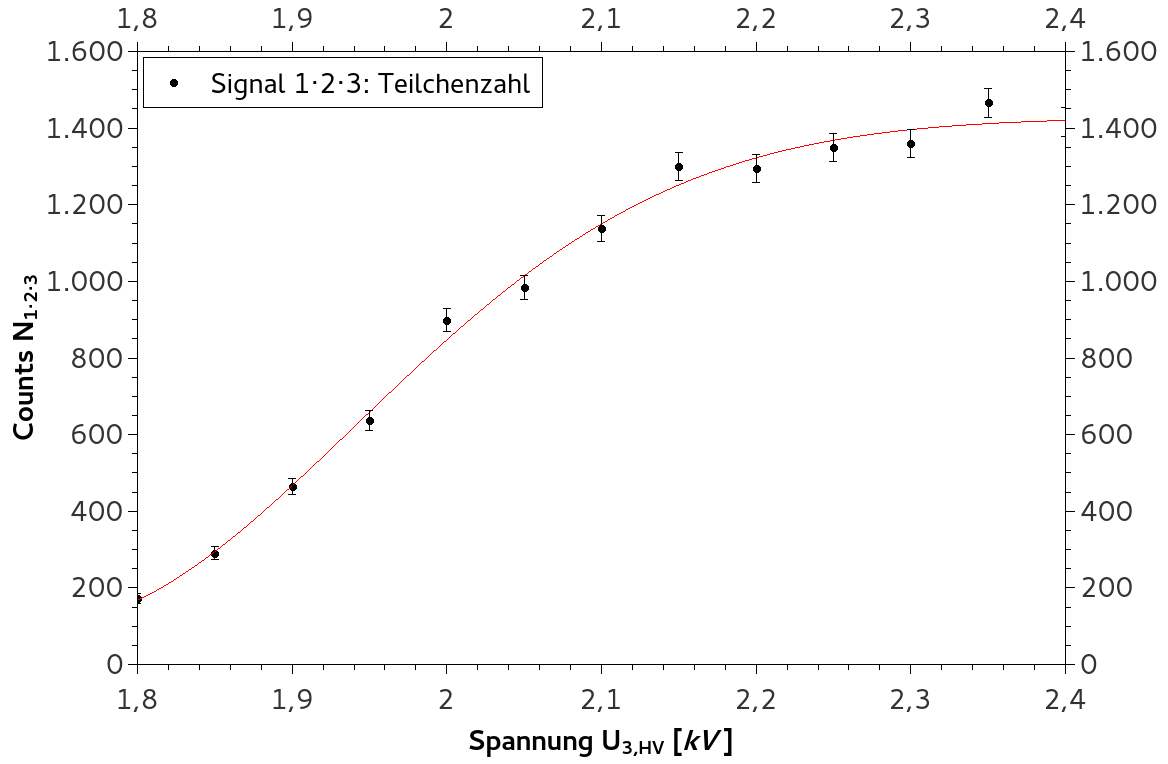
\includegraphics[scale=0.225]{pic/n123u3th}}
            \subfigure[Kennlinie des Signals $N_3$\label{n3}]{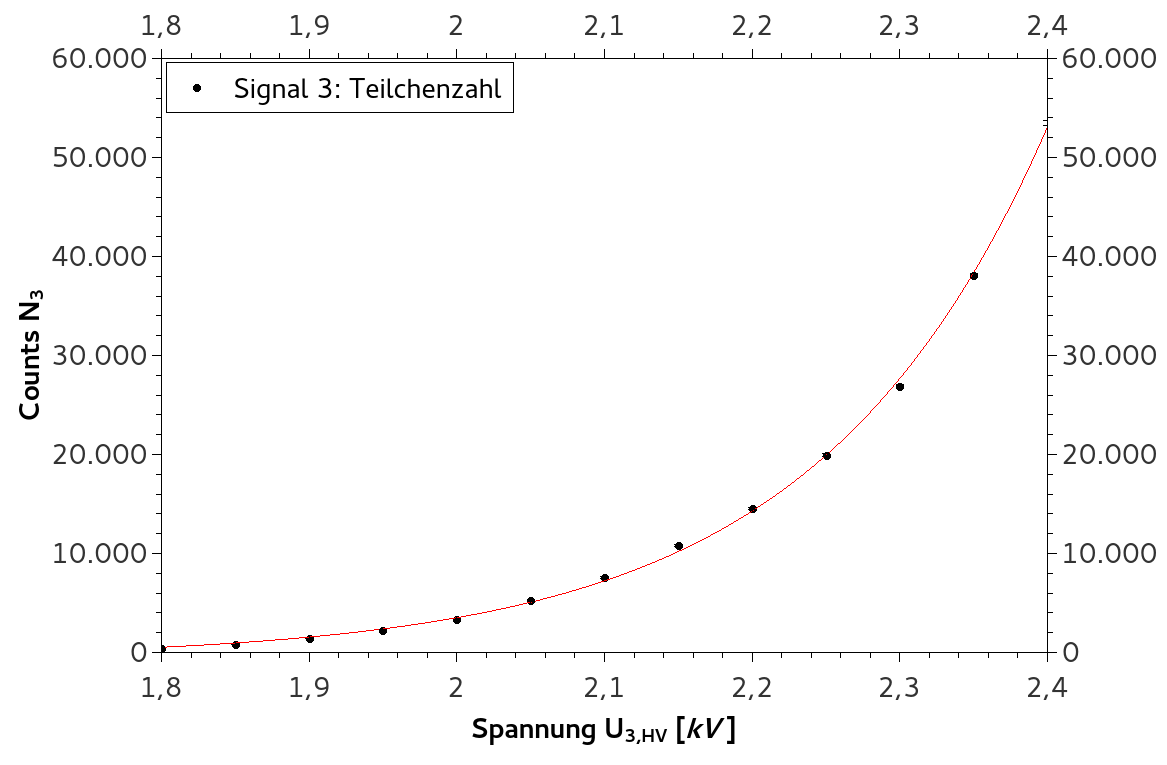
\includegraphics[scale=0.225]{pic/n3u3th}}
            \caption{Kennlinien der Hochspannung $U_{3,HV}$}
        \end{figure}
        Die Abbildungen \ref{n123} und \ref{n3} sehen sehr verschieden aus. Es ist stark auffällig, dass es sich bei \ref{n3} um ein exponentielles Wachstum handelt, während sich in \ref{n123} ein Plateau herausbildet, dessen verhalten eher einer kummulativen Verteilungsfunktion der Gauß-Kurve ähneln. 
        Die Unterschiede rühren vorallem daher, dass in \ref{n123} eine Triplezählrate vorliegt, für die Signale von allen Photomultipliern notwendig sind, um einen Count zu zählen. In \ref{n3} handelt es sich um eine Singlezählrate, die jeweils nur einen den Photomultiplier 3 misst, dessen Hochspannung man verändert. Je höher die Spannung ist, desto mehr Signale können detektiert werden. 